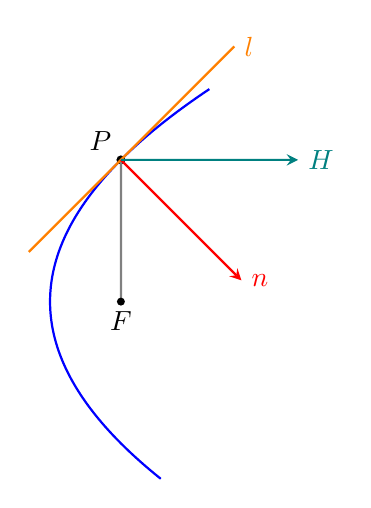
\begin{tikzpicture}[scale=.9,>=stealth]
\draw[blue,thick,domain=-2.5:3,samples=90] plot ({\x*\x/4},\x);
\coordinate (P) at (1,2);\fill (P) circle (1.8pt) node[above left] {$P$};
\draw[gray,thick] (P)--(1,0);\fill (1,0) circle (1.6pt) node[below] {$F$};
\draw[orange,thick] (-0.30000000000000004,0.7)--(2.6,3.6) node[right] {$l$};
\draw[->,red,thick] (P)--(2.7,0.30000000000000004) node[right] {$n$};
\draw[->,teal,thick] (P)--(3.5,2) node[right] {$H$};
\end{tikzpicture}
